\paragraph{}This chapter goes over the topic of SLAM, its subtypes and metrics, as well as the topic of hyperparameter optimization and its specific relevance in the context of SLAM optimization. Finally, related relevant work is discussed, so as to provide a context and a starting point for the work developed in this thesis.

\section{\ac{SLAM}}

\paragraph{}\ac{SLAM} is a fundamental problem in robotics and computer vision, wherein a system builds a map of an unknown environment while simultaneously determining its own position within said map\citep{taheri2021slam}.
\paragraph{}SLAM systems use sensors such as LIDAR's, cameras, IMU's and GPS to collect data about the environment, which then is processed by the backend itself\cite{taheri2021slam}, which is implementation dependent.
\paragraph{}Generally speaking, a SLAM method involves the following steps(not necessarily in this order):
\begin{itemize}
    \item Sensor data collection
    \item Feature extraction, to identify key features like landmarks, corners or edges
    \item Data association, where features from different sensor readings are matches with one another to better understand motion
    \item Pose estimation, where the position and orientation of the device within the environment is determined
    \item Map building - Using the sensor data extracted previously, a map of the environment is constructed and dynamically updated
    \item Loop closure - By recognizing previously visited locations, it is possible to correct some errors, such as drift
\end{itemize}

\subsection{Types of SLAM solutions}
\paragraph{}If one were to categorize SLAM solutions using the sensor types as a criteria, three broad categories would emerge: Visual SLAM(VSLAM), LiDAR SLAM, Radar SLAM and multi sensor SLAM.

\subsubsection{Visual SLAM}
\paragraph{}VSLAM uses cameras to understand an environment by detecting and tracking features over time\cite{chen2018review}. Common subtypes of VSLAM are(according to the type of cameras they use): Monocular SLAM, which uses only one camera, Stereo SLAM, which uses 2 cameras, separated by a known baseline, and RGB-D SLAM, which uses cameras that in addition to visual and color information, also provide pixel depth data(distance from camera to an object).
\begin{figure}[h]
    \centering
    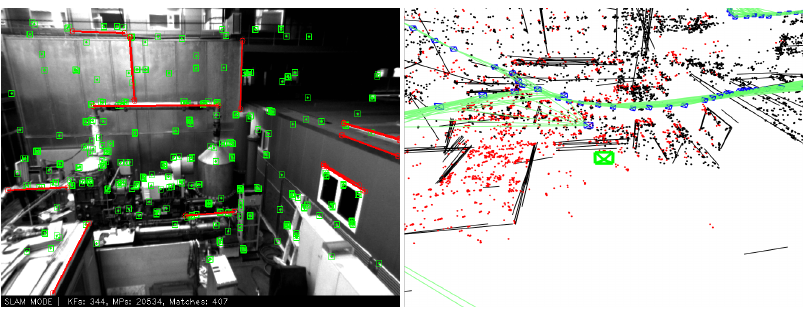
\includegraphics[width=0.75\linewidth]{images/VSLAM.png}
    \caption{Visual SLAM}
    \label{fig:enter-label}
\end{figure}

\paragraph{}In terms of system parameters, one has to consider those related to the different parts of the system, such as:
\begin{itemize}
        \item Feature detection and matching 
            \begin{itemize}
                \item feature matching threshold
                \item feature detection sensitivity
                \item scale factor(in case of pyramid-based detectors)
            \end{itemize}
        \item Pose/Motion estimation
            \begin{itemize}
                \item RANSAC threshold
                \item Number of RANSAC iterations, which affect the robustness and speed of the algorithm
                \item Minimum inliers, to control how many inliers before an estimated pose is accepted
            \end{itemize}
        \item Mapping
            \begin{itemize}
                \item Keyframe insertion threshold, which controlls how different a frame must be to be added as a keyframe
                \item Map point culling threshold, the criteria for removing bad or unused key points
            \end{itemize}
        \item Loop closure
            \begin{itemize}
                \item Minimum time between loops
                \item Loop detection threshold, level of confidence required to accept a loop
            \end{itemize}
\end{itemize}
\paragraph{}It should be noted that these parameters are only a fraction of the total number of parameters at play in VSLAM solutions, and are only briefly mentioned here. Also, other, more \textit{exotic}, less used algorithms might be used throughout the execution of the algorithm, which requires a different set of hyperparameters that those presented previously.

\subsubsection{LiDAR SLAM}
\paragraph{}LiDAR SLAM uses, as the name suggests, LiDAR(Light detection and ranging) sensors, which unlike VSLAM, can measure distances directly using laser pulses. It is overall a more robust method for low light and featureless environments.\cite{lidar_sota}
\begin{figure}[h]
    \centering
    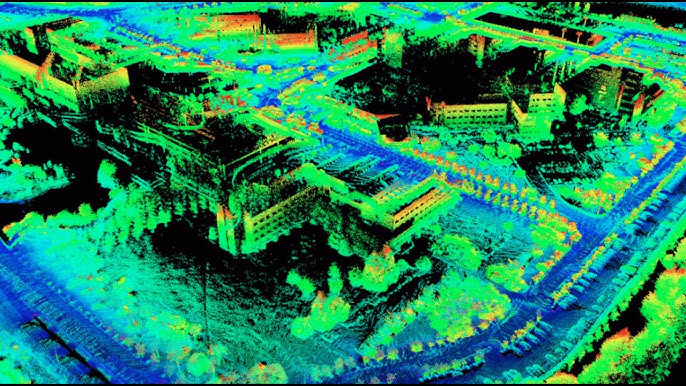
\includegraphics[width=0.75\linewidth]{images/lidar_SLAM.jpg}
    \caption{LiDAR SLAM point cloud example}
    \label{fig:enter-label}
\end{figure}
\paragraph{}In terms of system parameters, LiDAR solutions require preprocessing, introducing important parameters, such as Voxel grid size(Resolution for downsampling the point cloud) or the range threshold(range for keeping/eliminating points)\cite{lidar_sota}. As for the scan registration/motion estimation part of the method, according to the scan registration algorithm used(\ac{ICP}, \ac{NDT}, or other), different parameters will be used\cite{lidar_sota}.

\subsubsection{Radar SLAM}
\paragraph{}Radar SLAM uses radar sensors that gather data by emitting electromagnetic waves and analyzing their reflections on surrounding objects. This is particularly useful in adverse weather conditions, where Visual SLAM doesn't work as well\cite{hong2021radar}. However, it also has some serious limitations. For starters, a radar can't capture detailed structures the way a camera or lidar can. There is also the problem of lower resolutions, when compared to technologies like LiDAR\cite{radar_slam}. Due to these limitations, Radar is usually accompanied by other sensors, such as IMU or cameras of some type, making the overall SLAM system a \textbf{Multi sensor} system and taking advantage of the strengths of each sensor for a more robust map and trajectory estimation.
\begin{figure}[h]
    \centering
    %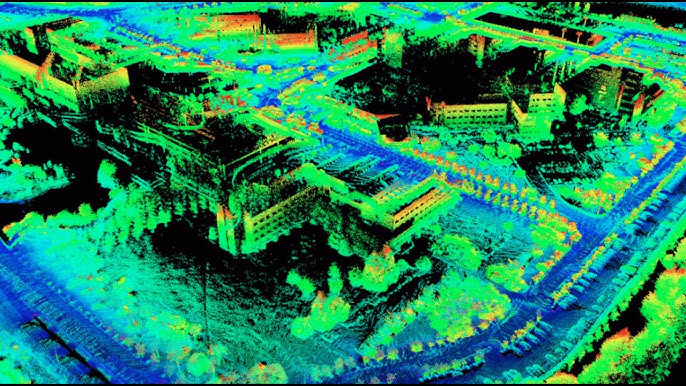
\includegraphics[width=0.75\linewidth]{images/lidar_SLAM.jpg}
    \includesvg[width=0.65\linewidth]{images/radar_slam.svg}
    \caption{Multi sensor SLAM system based on radar}
        \label{fig:enter-label}
\end{figure}

\subsubsection{Multi sensor SLAM}
\paragraph{}Multi sensor SLAM is simply a category for the \ac{SLAM} solutions which make use of several different types of sensors, taking advantage of the strengths of each one, making the final map and trajectories more robust than if each sensor was used on a independent \ac{SLAM} system.
\begin{figure}[h]
    \centering
    %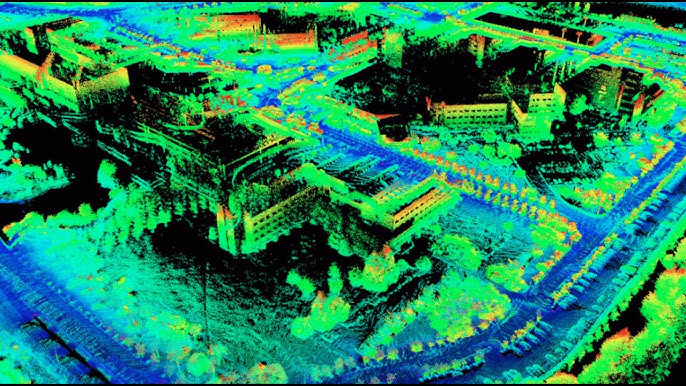
\includegraphics[width=0.75\linewidth]{images/lidar_SLAM.jpg}
    \includesvg[width=0.75\linewidth]{images/multisensor_slam.svg}
    \caption{Multi sensor SLAM system for an industrial robot}
    \label{fig:enter-label}
\end{figure}

\paragraph{}A few common multi sensor \ac{SLAM} sensor configurations include:
\begin{itemize}
    \item camera + IMU(Visual Inertial \ac{SLAM})\cite{visual_inertial} Cameras have good spatial information but low temporal resolution, while IMUs have high temporal resolution. When IMU accumulates too much drift, the cameras help correct it, and the IMU helps when vision is low. Main disadvantage is the high sensitivity to visual degradation(fog, dark areas, etc).
    \item Lidar-Inertial SLAM (LI-SLAM)\cite{liu2024voxelslamcompleteaccurateversatile}. Main advantage is the high robustness in low light or outdoor environments and the resilience to visual noise, present in nightly, foggy and even dusty environments. Two main limitations are the more expensive/heavier setups and the limitation in texture representation(pure geometry only).
    \item Visual-Lidar-Inertial SLAM (VLI-SLAM)\cite{liu2023lidarinertialvisualslamloopdetection}. In this approach, each sensor fills the gaps of the other, combining rich visual features, accurate range data, and motion tracking. Its main advantage lie in the high robustness and accuracy across varying environments. However, It requires a complex calibration and synchronization process, is expensive and requires more computational power than more simple multi sensor approaches to \ac{SLAM}.
\end{itemize}

\subsection{Evaluation of SLAM}
\paragraph{}Assessing SLAM performance requires quantitative and qualitative metrics that evaluate how accurate, robust and efficient the estimated map and trajectory are. A few evaluation criteria include:

\begin{itemize}
    \item Absolute Trajectory Error(\textbf{ATE}) - measures the global deviation between estimated and ground truth trajectories. At each point in the trajectory, the difference between the estimated pose and the ground truth pose is computed. For a more general measure of the ATE, one might also calculate the RMSE, as follows: 
    \begin{center} 
        \begin{equation} 
            ATE_{RMSE} = \sqrt{\frac{1}{N}\sum_{i=1}^{N}\|S(p_i^{est}) - p_i^{gt}\|^2}
        \end{equation}
    \end{center}
    \item Relative Pose Error(\textbf{RPE}) - measures the local consistency of the trajectory by evaluating the difference in relative motion between estimated and ground truth poses over a fixed time interval. As with ATE, the formula for the RMSE of the RPE is as follows:
    \begin{center}
        \begin{equation}
            RPE_{RMSE} = \sqrt{\frac{1}{N}\sum_{i=1}^{N}\|(T_i^{est})^{-1}T_{i+\Delta t}^{est} - (T_{i}^{gt})^{-1}T_{i+\Delta t}^{gt}\|^2}
        \end{equation}
    \end{center}
    \item Resource usage(memory, CPU) - taking into account resource utilization is an important aspect when comparing different SLAM methods, due to the trade-offs between accuracy and memory usage. In some applications, it might not be worth it to use a more computationally intensive(but more accurate) SLAM solution.
    \item Benchmarking - When evaluating and comparing different SLAM solutions, it is important to establish a fair playing field for all the algorithms to be compared. One of the ways to do that is to use publicly available standardized datasets, such as the KITTI Dataset. As for evaluation frameworks, one of the most widely used is EVO, which provides error metrics and visualization tools, so as to better compare the performance of different SLAM solutions.
\end{itemize}

\section{Hyperparameter optimization techniques}
\paragraph{}Hyperparameter optimization techniques can be broadly categorized into search-based, model-based and population-based approaches. Each approach uses different strategies to search the parameter space and obtain an approximation of the optimal solution, such as randomly sampling configurations(random search), mimicking physical processes to get a faster convergence(Simulated Annealing) or even by predefining a parameter space and drop half of the worst performing configurations at each pass(successive halving). Some of these approaches require a budget to be defined, meaning a time limit, or a maximum number of configurations to be tested.

\subsection{Search based approaches}
\paragraph{}One popular type of approach to the problem of HPO, which will be used as a baseline on this thesis' work, is a search based approach, such as Grid Search and Random Search. These approaches are popular due to their implementation simplicity and paralelization possibilities.
\subsubsection{Grid Search}
\paragraph{}Grid Search is a basic solution for Hyperparameter Optimization(HPO). It simply consists of an exhaustive search and evaluation of all possible hyperparameter combinations within a predefine parameter space\cite{yang2020hyperparameter}. In spite of the development of more specific algorithms in recent decades, Grid Search remains popular due to its simple implementation and trivial paralelization\cite{yang2020hyperparameter}. The main drawback is its computational cost, due to the curse of dimensionality being a serious problem in models with large numbers of hyperparameters\cite{yang2020hyperparameter}. This might be summarized by the following equation:

\begin{equation}
    N_c = \prod_{n=1}^{k} {N_{P_i}}
\end{equation}

where $N_c$ is the total number of configurations and $N_{P_i}$ is the number of possible values for hyperparameter i of the model.

By looking at \textbf{equation 2.1}, it becomes clear this algorithm is not very scalable, due to the rapid increase in the number of configurations, which makes this the main hurdle in search based approaches. One way of getting around it is paralelizing the execution of various configurations across several CPU cores and threads. Another way is to pre-select the parameters to optimize, and/or discarding hyperparameters which have little effect on the model's performance.

\begin{figure}[h]
    \centering
    %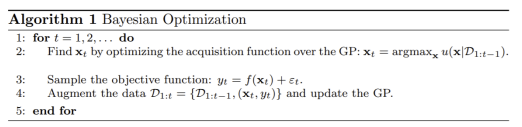
\includegraphics[width=0.75\linewidth]{images/BO.png}
    \includesvg[width=0.5\linewidth]{images/grid_search.svg}
    \caption{Graphical illustration of parameter space exploration in grid search}
    \label{fig:enter-label}
\end{figure}

\subsubsection{Random Search}
\paragraph{}Random Search is a variation of Grid Search. It randomly samples configurations in the aforementioned parameter space\cite{bissuel2020hyper}. Both Grid Search and Random Search are very similar implementation wise, with one major difference: Random Search requires a budget be specified, whether it is time, number of configurations, etc.\cite{bergstra2012random} The main advantage Random Search has over Grid Search is the faster convergence over a local or global optima\cite{bergstra2012random}, although this advantage gets slimmer the larger the parameter space.

\begin{figure}[h]
    \centering
    %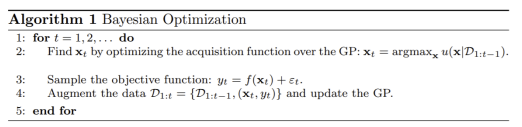
\includegraphics[width=0.75\linewidth]{images/BO.png}
    \includesvg[width=0.5\linewidth]{images/random_search.svg}
    \caption{Graphical illustration of parameter space exploration in random search}
    \label{fig:enter-label}
\end{figure}

\subsection{Model based approaches}
\paragraph{}Model based approaches tackle the optimization problem in a different way, by building a surrogate model that describes the relationship between hyperparameter configurations and algorithm performance. The inner workings of the algorithm to be optimized are unimportant and it is therefore treated as a black box. These kind of HPO techniques favor more complex optimization problems and clarify the relationship between algorithm performance and hyperparameter settings, which might prove to be a good option to pre select the most important hyperparameters to optimize when there are dozens or hundreds of parameters to optimize.
\subsubsection{Bayesian Optimization}
\paragraph{}\ac{BO} is a probabilistic model-based approach that optimizes black box functions that are expensive to evaluate\cite{mockus1998application}. It's particularly useful when the objetive function lacks an analytic expression and its evaluations are very expensive, which is the case for SLAM methods.


\begin{figure}[h]
    \centering
    %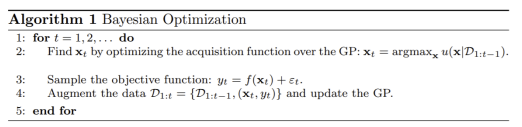
\includegraphics[width=0.75\linewidth]{images/BO.png}
    \includesvg[width=0.75\linewidth]{images/BO.svg}
    \caption{The Bayesian Optimization algorithm.}
    \label{fig:enter-label}
\end{figure}

\paragraph{}This method has two components:
\begin{itemize}
    \item Surrogate model that aproximates the objetive function, and is much easier to evaluate than the actual function\cite{elshawi2019automated}. Although multiple models can be used for this purpose, the most commonly used(and the standard) is Gaussian Processes(GP)\cite{bissuel2020hyper}.
    \item An aquisition function, that measures the value generated by evaluating the objective
function at a given point, and guides the search for the next point to evaluate\cite{elshawi2019automated}. It balances exploration(areas with high uncertainty) with exploitation(areas with high predicted performance). A few common aquisition functions include Expected Improvement(EI), Probability of Improvement(PI) and Upper Confidence Bound(UCB).
\end{itemize}

\paragraph{}\ac{BO} uses the following iterative process to optimize the objetive function:
\begin{enumerate}
    \item Select the next point to be sampled with the aquisition function.
    \item Evaluate the true function $f(x_1, x_2 ... x_n)$ at the selected point.
    \item Update the surrogate model with the new information using gaussian process regression, which is the process of adding additional information of the sampled points to the \textbf{prior}.
    \item Repeat steps 1, 2 and 3 until some stopping criteria is met(exhausted budget, achieved convergence, etc).
\end{enumerate}

\paragraph{}One major drawback of Bayesian Optimization is the impossibility of paralelization when compared to other baseline techniques, due to the fact the the surrogate model uses new points to update its parameters, meaning the learning process needs to finish before a new one can be launched\cite{bissuel2020hyper}.

\subsection{Population based Approaches}
\paragraph{}These types of approaches are defined by a population of candidate solutions(sets of hyperparameters) that are iteratively updated to optimize an objetive function\cite{kostusiak2019efficiency}, such as APE or RPE in the case of SLAM optimization.
\paragraph{}Population-based approaches are stochastic in nature. The specific techniques used in this thesis' work favor early exploration and become more exploitative over the course of the execution of the algorithm.

\subsubsection{Simulated Annealing}
\paragraph{}\ac{SA} is an optimization technique that mimicks the physical process of heating a metal and then cooling it slowly\cite{rutenbar1989simulated}. Analogously, the algorithm freely explores solutions in the beginning, even ones that seem worse at face value, so as to maximize exploration, and then, as the temperature decreases, according to a predefined cooling schedule, it focuses on refining a solution and maximizing exploitation.
\paragraph{}The method starts by assigning a single value to all hyperparameters, one that's supposed to be high enough to allow compreensive random search over the parameter space\cite{ghasemalizadeh2016review}. Then, it makes small changes to one parameter at a time and evaluates this new configuration, called a neighbor\cite{rutenbar1989simulated}. The aceptance of the neighbor as being the better solution depends on a probabilistic distribution, which in itself depends on the temperature and the difference between the current solution's and the neighbor solution's evaluation, like so:
\begin{gather*}
    P = e^{-\frac{\Delta E}{T}}
\end{gather*}
where T is the current temperature and $\Delta E$ is the difference between the cost of the new solution(the neighbor's) and the cost of the current solution, that is, $\Delta E = f'(x) - f(x)$.
\paragraph{}Then, the algorithm updates the temperature, using the following expression: $T' = \alpha T$, where $\alpha$ is the cooling factor, which is usually given a value in the interval [0.8, 0.99].
\paragraph{}The algorithm repeats the previous steps until the temperatures reaches a minimum value or a stopping condition is triggered, such as a maximum number of iterations\cite{ghasemalizadeh2016review}. Once execution stops, the best solution is returned as an approximation to the actual optimal solution. Figure 2.8 shows a graphic representation of SA’s behavior.

\begin{figure}[h]
    \centering
    %\includegraphics[width=0.5\linewidth]{}
    \includesvg[width=0.4\linewidth]{images/SA.svg}
    \caption{A graphic representation of the simulated annealing algorithm}
    \label{fig:enter-label}
\end{figure}

\subsubsection{Successive Halving}
\paragraph{}\ac{SH} is an optimization method that efficiently allocates resources to the most promising configurations while reducing investment into less promising ones\cite{soper2021greed}. Similar to Simulated Annealing, this technique requires a budget be specified(execution time, number of iterations, etc.).
\paragraph{}At first, $n$ candidates are generated and evaluated, and the constrained resources are assigned equally to all configurations. Then, \textbf{the worst half of all configurations is discarded} and this process is repeated until only 1 configuration remains\cite{huang2019survey}. The hyperparameter configurations used in this method can be generated in a variety of different ways. One can define a parameter space similar to the one used in search-based approaches and use either Grid Search or Random Search to generate the desired number of configurations. There is also the possibility of manually selecting both the hyperparameters to optimize and their values. This latter approach, combined with prior knowledge-based sampling, might prove to be a better stretegy for selecting and generating the starting configurations, due to the sheer number of hyperparameters in most SLAM methods.

\begin{figure}[h]
    \centering
    %\includegraphics[width=0.5\linewidth]{}
    \includesvg[width=0.6\linewidth]{images/SH.svg}
    \caption{A graphic representation of the Successive Halving algorithm}
    \label{fig:enter-label}
\end{figure}

\newpage

\subsubsection{Hyperband}
\paragraph{}Hyperband is a more efficient technique that builds on the Successive Halving algorithm\cite{elshawi2019automated, }. By dynamically allocating computational resources, Hyperband quickly identifies promising configurations and discards ill-performing ones early on, saving both time and CPU time.
\paragraph{}Hyperband works as follows:
\begin{enumerate}
    \item Define a total Budget B and the proportion of configurations to evaluate at each rung, $\eta$. Also, a maximum budget R for a single rung is required\cite{falkner2018bohb}.
    \item Generate a large number of configuration\cite{falkner2018bohb, }s.
    \item Allocate a small initial budget to all configurations and perform the successive halving algorithm with one modification: halt its execution when only the top 1 / $\eta$ configurations remain, instead of halting when only the best configuration remains. Then, increase the budget for the remaining configurations\cite{falkner2018bohb}.
    \item Repeat step 3 until maximum budget R is reached or all configurations are exhausted, meaning only the best one remains\cite{falkner2018bohb}.
\end{enumerate}

By increasing the budget allocated to a decreasing number of configurations at each execution of the Successive Halving algorithm, Hyperband transitions from an exploration-focused method to an exploitation-focused one.

\begin{figure}[h]
    \centering
    %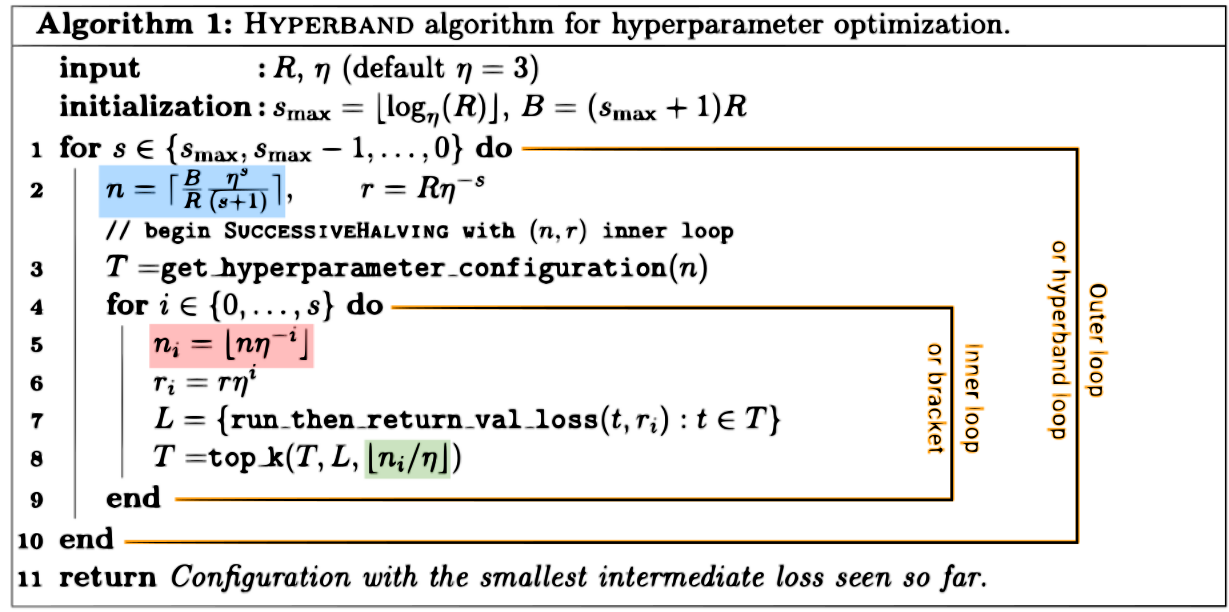
\includegraphics[width=0.5\linewidth]{images/Hyperband.svg}
    \includesvg[width=0.65\linewidth]{images/Hyperband.svg}
    \caption{\ac{HB} algorithm described in a more systematic way}
    \label{fig:enter-label}
\end{figure}

\newpage

\subsection{\ac{HPT} in \ac{SLAM}}
\paragraph{}When applying \ac{HPT} algorithms to fine tune a SLAM method's parameters, there are a few things to keep in mind.
\paragraph{}First, not all parameters are tunable. Better yet, some parameters have fixed or default values and are treated as constants during the tuning process, such as a camera's intrinsic parameters in VSLAM, or an IMU's noise and Bias models in Visual-Inertial \ac{SLAM}. This is an important aspect to keep in mind, especially when applying search based approaches, as it may provide a way to significantly reduce the number of configurations to be executed.
%\paragraph{}Another important topic when fine-tuning SLAM hyperparameters is benchmarking different HPO algorithms against each other. In this regard, both metrics and datasets are extremely important. On the one hand, metrics like ATE, RPE or IoU(Intersection over Union) might be all that is needed for certain applications. But it is also true that different HPO methods consume different amounts of system memory and take longer to execute. It is therefore a good strategy to take into account these metrics when deciding on a tuning strategy, depending on system resource constraints, time constraints, etc. As for the datasets, 
\paragraph{}As it pertains to the effectiveness of tuning strategies, search based methods are usually considered baseline methods in research, and not very effective when dealing with very high dimensional parameter spaces, as due to the high stochasticity of grid and random search. In this regard, simulated annealing achieves better results. But in order to obtain near optimal results

\section{Related Work}
\paragraph{}This subsection goes over published research in optimizing hyperparameters in \ac{SLAM} systems. It presents a brief description of each relevant article and the used \ac{SLAM} method and optimizing strategy, as well the results from the experiments that were made. It then goes over the current literature research gaps and presents the main contributions of this thesis.

\paragraph{}On search-based approaches, there has been some research on the topic. Particularly, authors have hand-selected and manually searched(brute force) the parameter space of a g-mapping SLAM solution\cite{ExampleArticle}. In this specific case, four parameters were tuned: linear\_update\_step, angular\_update\_step, quantity of particle, and resampling threshold. Through several executions of the algorithm, it was possible to reduce the navigation time of a robot from 32 seconds to 25 seconds.
\paragraph{}Another study applied grid search to optimize 5 parameters in a feature based monocular visual odometry setting\cite{zheng2020feature}. In all 10 sequences, measured ATE significantly decreased, showing the main advantage of this simple tuning approach. It is also worth noting that while search based approaches are more suited for a very reduced number of parameters, it is best to use grid search than manual search(brute force). While both papers presented previously show that, with good knowledge of the system, one can significantly reduce the parameter space down to the very few and impactful hyperparameters and obtain a near optimal configuration with both approaches.
\paragraph{}As far as model based approaches go, bayesian optimization is the most used algorithm in research. One paper used a variant of it, Sequential Model-Based Optimization (SMBO) to optimize the hyperparameters of a LiDAR Odometry algorithm, without knowledge of the  inner workings of the system, e.g the system is treated as a black box\cite{koide2021automatic}. Although data augmentation was used to prevent overfitting, it was still possible to observe a noticeable decrease in the odometry drift error(in most tested sequences). Another article, although outside the scope of this thesis, used Bayesian Optimization to fine tune the extrinsic parameters of a camera in a Visual Inertial SLAM sytem\cite{chen2018visual}.
\paragraph{}With regards to population-based approaches, there isn't much research in SLAM itself. However, one article explored the application of both a particle swarm algorithm and an evolutionary algorithm to optimize the parameters of an RGB-D Visual Odometry system \cite{kostusiak2019efficiency}. These meta-heuristics managed to reduce the execution time from several days to just a few hours, which is its main advantage. However, it is also concluded that these optimized parameters also generalize to other sequences, so long as camera dynamics(its intrinsic parameters) and execution environment stays the same.

\begin{landscape}
\begin{table}[h]
\centering
\begin{tabular}{|p{30mm}| p{30mm}| p{50mm}| p{75mm}|}
\hline
Article(s)                        & SLAM method                   & optimization method            & Results \\ \hline
Z. Zheng\cite{zheng2020feature}                          & Feature-based Visual Odometry & Grid Search                    &  Across 8 optimized sequences, average ATE decreased, on average, 64.68\%       \\ \hline
. A. Putra and P. Prajitno\cite{putra2019parameter}     & G-mapping SLAM                & Brute Force                    &  Navigation time of a predefined path was reduced from 32 to 25 seconds      \\ \hline
K. Koide et al\cite{koide2021automatic}                    & Lidar Odometry                & based on Bayesian Optimization & \textbf{With data augmentation}, in both tested environments, both components(translational and rotational) of the drift error decreased by at least 9.8\%.      \\ \hline
A. Kostusiak and P. Skrzypczyński\cite{kostusiak2019efficiency} & RGB-D Visual Odometry         & Particle Swarm Optimization    & Both ATE and RPE decreased by well over 50\%, and optimized parameters generalize well to other sequences        \\ \hline
A. Kostusiak and P. Skrzypczyński\cite{kostusiak2019efficiency} & RGB-D Visual Odometry         & Evolutionary Algorithm         &  optimization duration about 5x shorter than \ac{PSO},        \\ \hline
\end{tabular}
\caption{Summary of HPT methods used in the literature}
\label{tab:my-table}
\end{table}
\end{landscape}

\newpage

\subsection{Literature gaps}
\paragraph{}A few notable research gaps exist in the field of SLAM \ac{HPT}. Most notably:

%Research does not focus often enough on optimizing complete SLAM solutions. There is little exploration of meta-heuristics, which proved to have potential \cite{kostusiak2019efficiency}. There is also an abundance of search-based methods, such as grid search and manual search(brute force), which is to be expected, as most research papers focus only on one SLAM/Odometry system for a single, very particular use case. As such, knowledge of the inner workings of the system allows authors to pre select the most influential parameters and fixating the others, which exponentially decreases the size of the parameter space. However, more generalized and automatic approaches are lacking.

\begin{itemize}
    \item Lack of diversity in optimizing strategies. As presented earlier, most of the research use either a search based approach or a model-based approach(similar to \ac{BO}). In the case of the former, it is understandable. For \ac{SLAM} systems where there is a high degree of knowledge of the inner working of the sensors and how different parameters affect the performance of the solution, it is possible to manually set and stick with default values for some of the hyperparameters, and can then apply a simple baseline(search-based) approach to the tuning of the remaining hyperparameters. As for the latter, it is used most when there is no extensive knowledge of the system at hand. Therefore, \ac{BO} treats it as a black box and optimizes it. Apart from \cite{kostusiak2019efficiency}, there isn't much research on population-based approaches to optimizing \ac{SLAM}, whether variations of particle swarm algorithms, evolutionary algorithms, or more generally speaking, meta heuristics.
    \item Lack of a framework to automatically compare and optimize \ac{SLAM} method, allowing for an even playing field in \ac{SLAM} research. although RUSTLE, the tool which will built and improved upon during the course of this thesis, already allows for a somewhat organized approach to testing and optimizing complete \ac{SLAM} solutions, it lacks any automatic optimizing feature, meaning the only way to currently approach \ac{HPT} in RUSTLE is a brute force algorithm.
\end{itemize}

\subsection{Statement of contributions}
\paragraph{}Given that academic research often focuses on a single optimization method for a particular \ac{SLAM} system for an even more specific use case, the main contribution of this thesis is to widen the spectrum of optimization approaches to \ac{SLAM}, as well as allow for the automatic testing(optimization) of many different \ac{SLAM} solutions in an organized and systematic manner.